\documentclass{beamer}

% Code Segments
\usepackage{listings}
% Copyright 2017 Sergei Tikhomirov, MIT License
% https://github.com/s-tikhomirov/solidity-latex-highlighting/

\usepackage{listings, xcolor}

\colorlet{punct}{red!60!black}
\definecolor{background}{HTML}{EEEEEE}
\definecolor{delim}{RGB}{20,105,176}
\colorlet{numb}{magenta!60!black}

\lstdefinelanguage{json}{
    basicstyle=\normalfont\ttfamily,
    numbers=left,
    numberstyle=\scriptsize,
    stepnumber=1,
    numbersep=8pt,
    showstringspaces=false,
    breaklines=true,
    frame=lines,
    backgroundcolor=\color{background},
    literate=
     *{0}{{{\color{numb}0}}}{1}
      {1}{{{\color{numb}1}}}{1}
      {2}{{{\color{numb}2}}}{1}
      {3}{{{\color{numb}3}}}{1}
      {4}{{{\color{numb}4}}}{1}
      {5}{{{\color{numb}5}}}{1}
      {6}{{{\color{numb}6}}}{1}
      {7}{{{\color{numb}7}}}{1}
      {8}{{{\color{numb}8}}}{1}
      {9}{{{\color{numb}9}}}{1}
      {:}{{{\color{punct}{:}}}}{1}
      {,}{{{\color{punct}{,}}}}{1}
      {\{}{{{\color{delim}{\{}}}}{1}
      {\}}{{{\color{delim}{\}}}}}{1}
      {[}{{{\color{delim}{[}}}}{1}
      {]}{{{\color{delim}{]}}}}{1},
}

\lstset{
  language=json,
  escapeinside={<@}{@>},
	backgroundcolor=\color{verylightgray},
	extendedchars=true,
	basicstyle=\footnotesize\ttfamily,
	showstringspaces=false,
	showspaces=false,
	numbers=left,
	numberstyle=\footnotesize,
	numbersep=9pt,
	tabsize=2,
	breaklines=true,
	showtabs=false,
	captionpos=b
}


% Images
\usepackage{graphicx}

% Sequence Diagram
\usepackage{geometry}
\usepackage{pgf-umlsd}
\usetikzlibrary{calc}

\usecolortheme{beaver}

\AtBeginSection
{
  \begin{frame}
    \frametitle{Table of Contents}
    \tableofcontents[currentsection]
  \end{frame}
}

\setbeamertemplate{itemize items}{\textbullet}
\setbeamertemplate{footline}[text line]{%
  \parbox{\linewidth}{\vspace*{-8pt}
    \insertshorttitle\hfill\insertshortauthor\hfill\insertframenumber
  }
}
\setbeamertemplate{navigation symbols}{}

\begin{document}

\title{Alternative scalable HIDS with investigation capability}
\subtitle{FIDS - Forensic-based Intrusion Detection System}
\author{Julian Stampfli}

\frame{\titlepage}


\begin{frame}
  \frametitle{Table of Contents}
  \tableofcontents
\end{frame}

%%%%%%%%%%%%%%%%%%%%%%%%%%%%%%%%%%%%%%%%%%%%%%%%%%%%%%%%%%%%%%%%%%%%%%%%%%%%%%%%
\section{Introduction}
%%%%%%%%%%%%%%%%%%%%%%%%%%%%%%%%%%%%%%%%%%%%%%%%%%%%%%%%%%%%%%%%%%%%%%%%%%%%%%%%

\begin{frame}[fragile]
  \frametitle{Intrusions}
  \begin{itemize}
    \item What?
    \begin{itemize}
      \item Malware
      \item Hacker
      \item Insider Threats
    \end{itemize}
    \pause
    \item Protection 
    \begin{itemize}
      \item Firewals
      \item Least privilege
      \item ...
    \end{itemize}

    \item Secure\pause ?
    \begin{itemize}
      \item Open Ports
      \item Weak Passwords
      \item Insecure Applications
      \item ...
    \end{itemize}
  \end{itemize}
\end{frame}

\begin{frame}[fragile]
  \frametitle{Intrusion Detection}
  \begin{columns}
    \begin{column}{0.5\textwidth}
      Network-Based
      \begin{itemize}
        \item Central scanning
        \item Uses
        \begin{itemize}
          \item Traffic Load
          \item Connections
          \item Inspection
        \end{itemize}
        \item Mainly pattern driven
      \end{itemize}
    \end{column}
    \begin{column}{0.5\textwidth}
      Host-Based
      \begin{itemize}
        \item Distributed Scanning 
        \item Uses
        \begin{itemize}
          \item Processes
          \item Files
          \item Network Configuration
        \end{itemize}
        \item Change driven
      \end{itemize}
    \end{column}
  \end{columns}
\end{frame}

\begin{frame}[fragile]
  \frametitle{HIDS - FIM}
  \begin{columns}
    \begin{column}{1\textwidth}
      Finding Changes
      \begin{itemize}
        \item Hashing to the rescue! \pause or not?
      \end{itemize}
    \end{column}
  \end{columns}
\end{frame}

\begin{frame}[fragile]
  \frametitle{Hashing}
  \begin{columns}
    \begin{column}{1\textwidth}
      \begin{itemize}
        \item Highly reliable
        \item Used for cryptographic use cases
        \item Fast? \pause - Yes but not really.
        \item FIM using Hashing?
        \begin{itemize}
          \item Tripwire - 1992 - Gone comercial
          \item Aide / Samhain - Current Opensource alternatives
        \end{itemize}
      \end{itemize}
    \end{column}
  \end{columns}
\end{frame}


\begin{frame}[fragile]
  \frametitle{HIDS - FIM}
  \begin{columns}
    \begin{column}{1\textwidth}
      Finding Changes
      \begin{itemize}
        \item Hashing
        \item Filesystem attributes to the rescue
      \end{itemize}
    \end{column}
  \end{columns}
\end{frame}

\begin{frame}[fragile]
  \frametitle{TSK}
  \begin{columns}
    \begin{column}{1\textwidth}
      The Sleuth Kit.
      \begin{itemize}
        \item Opensource
        \item Disk analyzis utility
        \item Used in forensics
      \end{itemize}
    \end{column}
  \end{columns}
\end{frame}

%%%%%%%%%%%%%%%%%%%%%%%%%%%%%%%%%%%%%%%%%%%%%%%%%%%%%%%%%%%%%%%%%%%%%%%%%%%%%%%%
\section{Forensic-based Intrusion Detection System (FIDS)}
%%%%%%%%%%%%%%%%%%%%%%%%%%%%%%%%%%%%%%%%%%%%%%%%%%%%%%%%%%%%%%%%%%%%%%%%%%%%%%%%


\begin{frame}[fragile]
  \frametitle{FIDS - Architecture}
  \begin{columns}
    \begin{column}{1\textwidth}
      \begin{figure}[ht]
        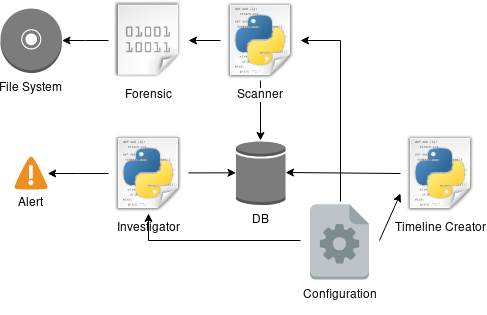
\includegraphics[width=8cm]{../img/Overview_FIDS.png}
        \centering
        \caption{System Architecture}
        \label{fig:systemArchitecture}
      \end{figure}
    \end{column}
  \end{columns}
\end{frame}

\begin{frame}[fragile]
  \frametitle{FIDS}
  \begin{columns}
    \begin{column}{1\textwidth}
      \begin{itemize}
        \item Scanner
        \begin{itemize}
          \item Collects Data from Files System through TSK
          \item Saves data to Database
        \end{itemize}
        \item Investigator
        \begin{itemize}
          \item Compares Runs
          \item Creates a list of anomalies
        \end{itemize}
        \item Timeline Creator
        \begin{itemize}
          \item ``Time Machine Format" (Forensic Timelining)
        \end{itemize}
      \end{itemize}
    \end{column}
  \end{columns}
\end{frame}

%%%%%%%%%%%%%%%%%%%%%%%%%%%%%%%%%%%%%%%%%%%%%%%%%%%%%%%%%%%%%%%%%%%%%%%%%%%%%%%%
\section{Summary/Conclusion}
%%%%%%%%%%%%%%%%%%%%%%%%%%%%%%%%%%%%%%%%%%%%%%%%%%%%%%%%%%%%%%%%%%%%%%%%%%%%%%%%

\begin{frame}[fragile]
  \frametitle{Conclusion}
  \begin{columns}
    \begin{column}{1\textwidth}
      Summary
      \begin{itemize}
          \item Fast Scans
          \item Intrusion Detection Possible
          \item Support for Forensic Investigation
      \end{itemize}
      \pause
      Conclusion
      \begin{itemize}
        \item Risk-Based Approach
        \item Speed vs Reliability
      \end{itemize}
    \end{column}
  \end{columns}
\end{frame}

\begin{frame}[fragile]
  \frametitle{Further Research}
    \begin{itemize}
      \item Extension beyond Files
      \item Extensive Testing in a Live Environment
    \end{itemize}
\end{frame}


\begin{frame}
  \frametitle{Thank you for listening / Demo?}
  Come to my booth.

  Code: \url{https://github.com/Tartori/fids}
\end{frame}

\end{document}
